\chapter{Controllability and observability}\label{chap:controlandobserve}

This lab will demonstrate the fundamental ideas behind the controllability
and observability properties of a system.  You will analyze a simple circuit
and determine the conditions for observability and controllability.  You will
then proceed to simulate the system using \textsf{Simulink} under various
conditions.

\section{Prelab}

You may wish to read Sections 2.3.1 and 2.3.2 from the
course notes to recall some background on controllability and observability.

Using Figure~\ref{fig:circuit}
\begin{figure}[htbp]
    \centering
    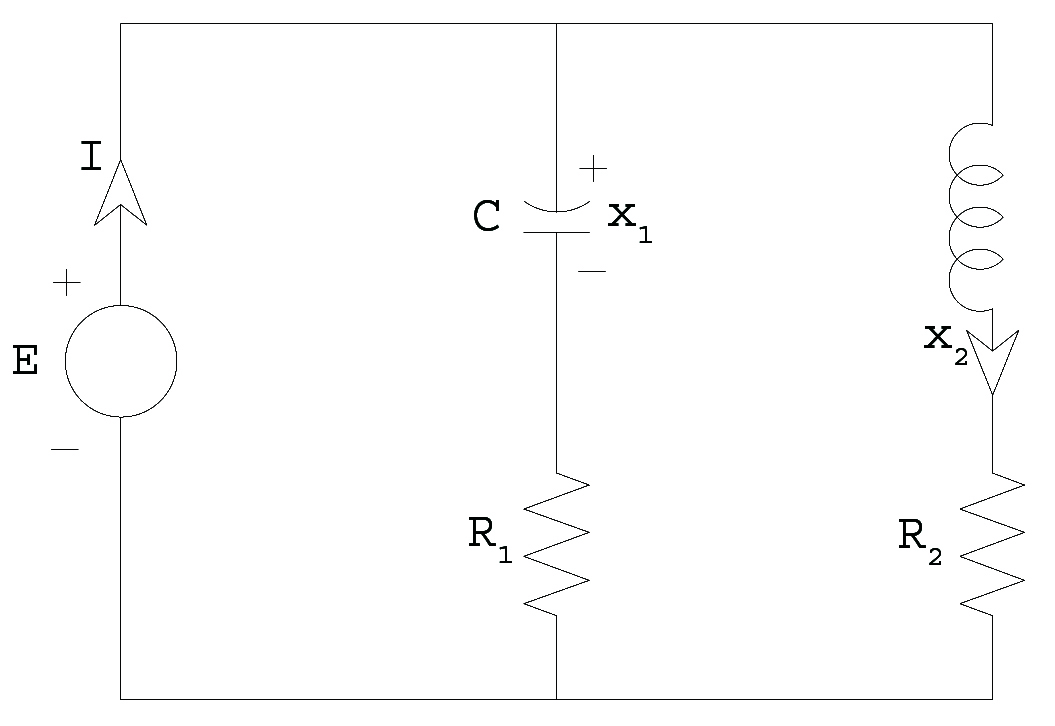
\includegraphics[width=0.6\hsize]{pix/circuitlarge.jpg}
    \caption{State space configuration}\label{fig:circuit}
\end{figure}
as a reference, define \(x_{1}\) as the voltage across the capacitor, and
\(x_{2}\) as the current through the inductor.  Take the output to be the
current entering the circuit, denoted \(I\) in Figure~\ref{fig:circuit}.

\begin{enumerate}
    \item Write out the system equations in the state-space form:
          \begin{eqnarray*}
              \dot{\vect{x}}=\mat{A}\vect{x}+\vect{b}u,\\y=\vect{c}^{t}+\mat{D}u.
          \end{eqnarray*}
          If you are having trouble getting the differential equations, or just not
          ``electrically inclined'', you should review past course notes on electrical
          circuits and differential equations.  Suck it up, Apple Mech students!
          \begin{itemize}
              \item When finding the differential equations for a system, your goal should
                    be to determine an expression for the derivative of each state variable in
                    terms of the state variable(s) and the forcing function.  Once you have %chktex 36
                    these, you can determine \(\mat{A}\) and \(\vect{b}\).

              \item The following facts may be useful.  The current through a capacitor is
                    given by \(I_{c}=C\frac{dV_{C}}{dt}\), the voltage across an inductor is
                    given by \(V_{L}=L\frac{dI_{L}}{dt}\), and the voltage across a resistor is
                    given by Ohm's law, \(V_{R}=I_{R}R\).  By Kirchoff's voltage law, the voltage
                    across each branch of the circuit is simply \(E\). You can use this fact to
                    get expressions for \(\mat{A}\) and \(\vect{b}\).

              \item Since the output is the current entering the circuit, and you will by
                    this point have expressions available for the current in each branch, you can
                    use Kirchoff's current law (i.e., conservation of current) to determine
                    expressions for \(\vect{c}\) and \(\mat{D}\).
          \end{itemize}

    \item Calculate the controllability matrix \(\mat{C}(\mat{A},\vect{b})\).

    \item Calculate the observability matrix \(\mat{O}(\mat{A},\vect{c})\).

    \item Determine the conditions under which the system is uncontrollable.
          Recall that a square matrix has full rank if and only if its determinant is
          non-zero.

    \item Determine the conditions under which the system is unobservable.

    \item When the system is uncontrollable, determine the set of reachable
          points for zero initial conditions.  This is going to be a one-dimensional
          vector space, so there is a simple relationship between \(x_{1}\) and \(x_{2}$.
          Determine this relationship when the system is uncontrollable.

    \item When the system is unobservable, determine the set of initial
          conditions that yield the same output, and the linear relationship between
          the initial conditions.
\end{enumerate}

\section{Procedure}

Via simulation, you will determine the conditions under which the circuit in
Figure~\ref{fig:circuit} is controllable and/or observable.

\subsection{Controllability}

When analyzing the controllability, you will be examining the behaviour of
the system states.  Recall that a rough definition of controllability is:
``starting from the origin, you can reach any point in state space by
applying an appropriate input.''
\begin{enumerate}
    \item Build the \textsf{Simulink} model as shown in
          Figure~\ref{fig:model2}.
          \begin{figure}[htbp]
              \centering
              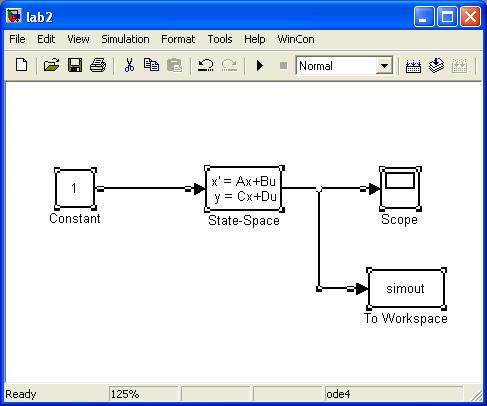
\includegraphics[width=0.6\hsize]{pix/controlandobservemodel.jpg}
              \caption{\textsf{Simulink} model for Lab~\ref{chap:controlandobserve}}\label{fig:model2}
          \end{figure}%
          The model applies a constant voltage to the dynamic model defined by
          \(\mat{A}\), \(\vect{b}\), \(\vect{c}\), and \(\mat{D}\) defined
          previously. The output is the current in the circuit.

    \item Define the matrices \(\mat{A}$\@, \(\vect{b}$\@, \(\vect{c}\), and
          \(\mat{D}\) by double-clicking on the \verb|State-space| block.  Each matrix is
          entered using the following convention. The following is an example on how to
          properly input values into the \verb|State-Space| block. The values shown are
          \emph{not} the proper values.  Use values that correspond to the matrices in
          the prelab.  The matrix
          \begin{equation*}
              \mat{A}=\begin{bmatrix}0&1\\-1&2\end{bmatrix}
          \end{equation*}
          is entered by typing \verb|[0,1;-1,-2]| in the line reserved for \(\mat{A}$\@.
              Note that elements of a row are delimited by comma (or spaces) and each row
              is delimited by a semicolon.

              The entries of Figure~\ref{fig:stateConfiguration}
              \begin{figure}[htbp]
                  \centering
                  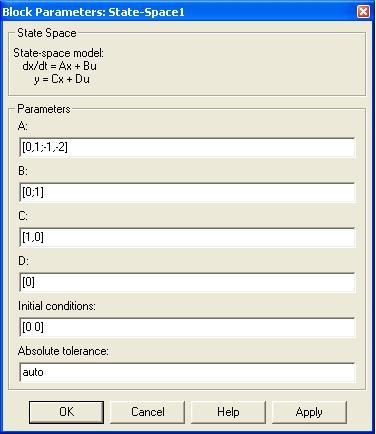
\includegraphics[width=0.6\hsize]{pix/controlandobserveentries.jpg}
                  \caption{State space configuration}\label{fig:stateConfiguration}
              \end{figure}%
              correspond to the dynamical system
              \begin{eqnarray*}
                  \dot{\vect{x}}&=&\begin{bmatrix}0&1\\-1&-2\end{bmatrix}\vect{x}
                  +\begin{bmatrix}0\\1\end{bmatrix}u,\\
                  y&=&\begin{bmatrix}1&0\end{bmatrix}\vect{x}+[0]u.
              \end{eqnarray*}
              Note that the last line specifies the initial conditions for the states.  In
              this case, we have set \(x_{1}(0)=0\) and \(x_{2}(0)=0$\@.  Come up with an
          appropriate variable to show the linear relationship between \(x_{1}\) and
          \(x_{2}\) when the system is uncontrollable (make sure you record this in your
          lab report).  Define this variable as one of your outputs in your model.
          Note that you can add as many outputs as you want just by adding rows to the
          matrix \(\vect{c}$\@.

          Define the initial conditions to be zero.  The default final time is set to
          10 by \textsf{Simulink}.  You may change it by opening the window
          \begin{center}
              \verb|Simulation|\(\rightarrow \)\verb|Configuration Parameters|
          \end{center}
          and entering the required time in the \verb|Stop Time| box.

    \item Run the \textsf{Simulink} block under uncontrollable conditions. This
          will depend on your choice of \(R_{1}\), \(R_{2}\), \(C\), and \(L\).
          Recuperate the state variable values written to the workspace and plot
          \(x_{1}\), \(x_{2}\), and the output variable you defined.  Does the output
          variable you chose show that there is, in fact, a linear relationship between
          \(x_{1}\) and \(x_{2}\)? Under these conditions, is it possible to find an input
          voltage \(E\) that will allow you to reach a point that is off this line?

    \item Add an appropriate title to your graph and print it.

    \item Rerun the system, but this time use conditions that make the system
          controllable.  Plot and print a graph of \(x_{1}\) and \(x_{2}\) and your output
          variable.  What can you now say about your output variable?  What is the set
          of reachable points under these conditions?

    \item Again, give an appropriate title to your graph and print it.
\end{enumerate}

\subsection{Observability}

When analyzing observability, you will be examining the output behaviour of
the system.  Recall that a rough definition of observability is: ``a change
in initial conditions and/or input results in a change in the output.''
\begin{enumerate}
    \item Using the work from your prelab, enter the value of \(\mat{A}\),
          \(\vect{b}\), \(\vect{c}\), and \(\mat{D}\) into the \verb|State-Space| block.
          Change the name of the output variable from \verb|simout| to \verb|I|.

    \item We will want to examine the output using many different initial
          conditions.  Build and run the system using a pair of initial conditions that
          are in the kernel of the observability matrix.  Plot, and print a graph of
          the output variable \(I$.  Make sure that you include values of the constants
          in the title of the plot.

    \item Rerun the system using a different pair of initial conditions that are
          also in the kernel of the observability matrix.  Include a plot of the
          output.  Does the result of this experiment confirm your work from the
          prelab? What happens if you use initial conditions that are not in the kernel
          of the observability matrix?
\end{enumerate}

When you have completed the lab, make sure you move the files created in the
directory created in Lab~\ref{chap:intro}.

%%% Local Variables: 
%%% mode: latex
%%% TeX-master: "lab-manual"
%%% End: 
